\documentclass[a4paper]{article}
 
% - taille de la fonte    : 10pt, 11pt, 12pt
% - recto ou recto-verso    : oneside, twoside
 
% Chargement d'extensions
%\usepackage[latin1]{inputenc}    
\usepackage[francais]{babel}    
\AtBeginDocument{\def\labelitemi{$\bullet$}}
%%%%%%%%%%%%%%%%%%%%%%%%%%%
\usepackage{amsthm}
\usepackage{amsmath}
\usepackage{amssymb}
\usepackage{mathrsfs}
\usepackage{graphicx}
\usepackage{geometry}
\usepackage{stmaryrd}
\usepackage{tikz}
\usetikzlibrary{patterns}

\usepackage[cache=false]{minted}
\usepackage{xcolor}
%\setbeamercolor{background canvas}{bg=lightgray}
\definecolor{LightGray}{gray}{0.9}
\definecolor{monOrange}{rgb}{0.97,0.35,0.04}

% Informations le titre, le(s) auteur(s), la date
\title{Les bases du CSS}
\author{Ibrahim ALAME}
\date{\today}
\includeonly{ introduction.tex} 
\begin{document}
 
\maketitle

\section{Présentation du chapitre}
\subsection{Rappels sur le {\color{monOrange}CSS}}
Les feuilles de style en cascade, pour {\color{monOrange}CSS (Cascading Style Sheets)} est un langage qui décrit la présentation des documents {\color{monOrange}HTML}. Le principe du {\color{monOrange}CSS} est de sélectionner certains éléments pour leur appliquer un style particulier.

\subsection{Les règles {\color{monOrange}CSS}}
Tout le {\color{monOrange}CSS} se divise a minima de cette manière si il n'est pas appliqué côté {\color{monOrange}HTML} (ce qui est déconseillé comme nous le verrons) :

\begin{center}
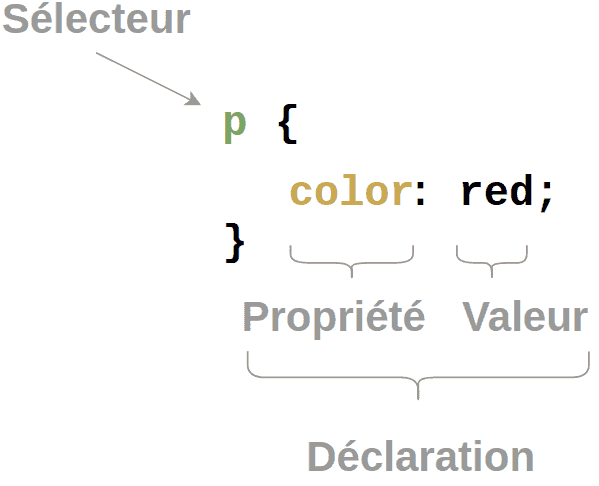
\includegraphics[width=10cm]{images/image07.png}
\end{center}

Le sélecteur permet de sélectionner le contenu {\color{monOrange}HTML} sur lequel la règle doit s'appliquer. Ici, par exemple, la règles s'appliquera à tous les éléments {\color{monOrange}HTML} p, c'est-à-dire à tous les paragraphes. Après le sélecteur, nous avons forcément une paire d'accolades qui contiennent la ou les propriétés à modifier pour les éléments sélectionnés. 
\begin{itemize}
\item La propriété est ce que l'on souhaite définir sur l'élément. Par exemple ici sa couleur. Il faut toujours utiliser : pour séparer la propriété et la ou les valeurs à lui donner.

\item La valeur est la mise en forme à appliquer pour une propriété donnée. Ici, de mettre la couleur en rouge. Il faut toujours terminer par ; pour passer à la modification suivante, par exemple :
\end{itemize}

\begin{minted}[
mathescape,
framesep=2mm,
baselinestretch=1.2,
%fontsize=\footnotesize,
bgcolor=LightGray,
%linenos
]{css}
p {
  color: red;
  width: 100px;
}
\end{minted}

\subsection{Comment le {\color{monOrange}CSS} fonctionne t-il ?}
Pour afficher un {\color{monOrange}document} le navigateur va réaliser les principales étapes suivantes :
\begin{enumerate}
\item  Il va charger le code {\color{monOrange}HTML} avec une requête {\color{monOrange}HTTP}.

\item  Il va convertir le {\color{monOrange}HTML} en objet l'{\color{monOrange}DOM (document object model)}. Il s'agit du modèle en arbre de tous les éléments {\color{monOrange}HTML} de la page qui est mis en mémoire vive pour pouvoir le modifier dynamiquement. Nous y reviendrons

\item   Le navigateur va récupérer toutes les ressources contenues dans les liens indiqués dans le {\color{monOrange}HTML} dont les feuilles de style {\color{monOrange}CSS}. Il effectue donc des requêtes {\color{monOrange}HTML} supplémentaires.

\item   Le navigateur analyse les règles {\color{monOrange}CSS} pour créer un arbre de rendu (ou render tree) qui contient tous les styles à appliquer aux différents sélecteurs.

\item   Enfin le navigateur affiche le {\color{monOrange}document} en prenant donc en compte le {\color{monOrange}HTML} et le {\color{monOrange}CSS} (et éventuellement le {\color{monOrange}JavaScript}, nous y reviendrons plus tard). Il s'agit de la phase de peinture ({\color{monOrange}painting}).
\end{enumerate}


\begin{center}
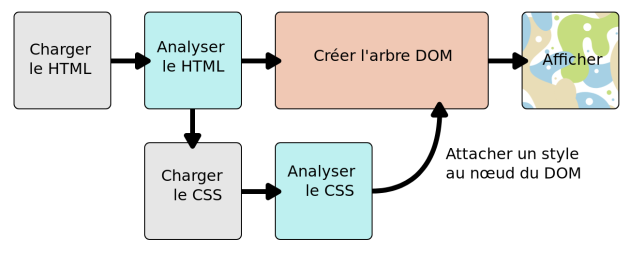
\includegraphics[width=10cm]{images/image08.png}
\end{center}

%%%%%%%%%%%%%%%%%%%%%%%%%%%%%%%%%%%%%%%%%%%%%%%%%%%%%%%%%%%%%%%%%%%%%%%%%%%%%%%

\section{Déclarer des règles CSS}
Il existe trois manière d'appliquer du {\color{monOrange}CSS} à un document {\color{monOrange}HTML}. Cependant une seule est recommandée et nous la verrons en dernier.

\subsection{Styles en ligne}
La première méthode est déconseillée mais vous serez amené à la voir souvent. Il s'agit de mettre du {\color{monOrange}CSS} directement dans le {\color{monOrange}HTML}. Par exemple :
\begin{minted}[
mathescape,
framesep=2mm,
baselinestretch=1.2,
%fontsize=\footnotesize,
bgcolor=LightGray,
%linenos
]{html}
<p style="color:red;">Element paragraphe avec du style CSS en ligne.</p>
\end{minted}
Ce n'est pas bon pour de nombreuses raisons :
\begin{itemize}
\item La première est qu'en programmation, un des concepts fondamentaux est la séparation des préoccupations. Cela signifie qu'il ne faut pas mélanger du code qui n'ont pas du tout les mêmes finalités. Ici le {\color{monOrange}HTML} est pour la structure du {\color{monOrange}document} et le {\color{monOrange}CSS} pour la mise en forme du {\color{monOrange}document}. Ils n'ont pas la même finalité et doivent donc être séparés.

\item Deuxième raison, la lisibilité et la maintenabilité du code s'en trouve fortement réduite car la combinaison de règles devient compliquer à comprendre et à mettre à jour. 
\item Troisième raison, l'un des autres concepts très important en programmation est de rester {\color{monOrange}DRY (don't repeat yourself)}. Cela signifie qu'il faut éviter au maximum de répéter le même code à différents endroits.
\end{itemize}
Ici, si vous voulez appliquer le même style à plusieurs paragraphes qui sont dans différents fichiers {\color{monOrange}HTML} ou dans des parties différentes vous devrez vous répéter. Cela aura pour conséquence de diminuer la maintenabilité du code car lors d'une mise à jour il faudra se rappeler tous les endroits où vous avez mis des règles {\color{monOrange}CSS}.

La seule exception est pour les emails car les clients de messagerie sont plus nombreux et moins bien développés que les navigateurs. Pour s'assurer que le {\color{monOrange}CSS} soit bien compatible avec tous les clients de messagerie, il est commun de mettre les règles {\color{monOrange}CSS} en ligne.

\subsection{Feuilles de style interne}
Une feuille de style interne est l'utilisation de règles {\color{monOrange}CSS} à l'intérieur de balises <style> dans le fichier {\color{monOrange}HTML} dans la partie {\tt <head>}. Pour les mêmes raisons, ce n'est pas recommandé.

Voici un exemple :
\begin{minted}[
mathescape,
framesep=2mm,
baselinestretch=1.2,
%fontsize=\footnotesize,
bgcolor=LightGray,
%linenos
]{html}
<!DOCTYPE html>
<html lang="fr">
  <head>
    <meta charset="UTF-8" />
    <meta name="viewport" content="width=device-width, initial-scale=1.0" />
    <meta http-equiv="X-UA-Compatible" content="ie=edge" />
    <title>Appliquer des styles CSS</title>
    <style>
      div {
        color: blue;
      }
    </style>
  </head>
  <body>
    <div>Div avec feuille de style interne</div>
  </body>
</html>
\end{minted}
\subsection{Feuilles de style externe}
Cette méthode permet l'utilisation de fichiers {\color{monOrange}CSS} externes. C'est la méthode recommandée. Vous pouvez facilement appliquer les mêmes styles dans plusieurs pages {\color{monOrange}HTML} en important la même feuille de styles dans les différents fichiers. Il suffit de créer un fichier {\color{monOrange}CSS} avec l'extension {\color{monOrange}.css} puis de l'inclure avec un élément {\color{monOrange}link} :
\begin{minted}[
mathescape,
framesep=2mm,
baselinestretch=1.2,
%fontsize=\footnotesize,
bgcolor=LightGray,
%linenos
]{html}
<!DOCTYPE html>
<html>
  <head>
    <meta charset="utf-8">
    <title>Feuille de styles externe</title>
    <link rel="stylesheet" href="styles.css">
  </head>
  <body>
    <p>Un paragraphe avec du contenu.</p>
  </body>
</html>
\end{minted}
Dans le fichier CSS, vous pouvez mettre directement les règles :
\begin{minted}[
mathescape,
framesep=2mm,
baselinestretch=1.2,
%fontsize=\footnotesize,
bgcolor=LightGray,
%linenos
]{css}
h1 {
  color: blue;
}

p {
  color: red;
}
Copier
\end{minted}
Voici un exemple avec les trois méthodes pour appliquer des styles {\color{monOrange}CSS} :

%%%%%%%%%%%%%%%%%%%%%%%%%%%%%%%%%%%%%%%%%%%%%%%%%%%%%%%%%%%%%%%%%%%%%%%%%%%%%%%

\section{Les classes, les ids et les sélecteurs}
\subsection{Les sélecteurs CSS}
Nous avons déjà vu ce qu'était un sélecteur : il permet de sélectionner un ou plusieurs éléments HTML sur lesquels appliquer une ou plusieurs règles CSS.

Cette leçon va être plus détaillée que la vidéo pour vous donner un aperçu approfondi des règles. Nous vous conseillons de les survoler pour le moment, nous y reviendrons au fur et à mesure dans les chapitres suivants.

Il existe différents types de sélecteurs : le sélecteur universel, les sélecteurs de type, les classes, les ids, les sélecteurs d'attribut, les combinateurs et les pseudo-classes.

Nous allons tous les voir sauf les pseudo-classes que nous verront plus tard.

\subsection{Le sélecteur universel *}
Le sélecteur universel permet d'appliquer des règles à tous les éléments de la page.
\begin{minted}[
mathescape,
framesep=2mm,
baselinestretch=1.2,
%fontsize=\footnotesize,
bgcolor=LightGray,
%linenos
]{css}
* {
  color: red;
}
\end{minted}
Vous vous en servirez rarement.

\subsection{Les sélecteurs de type}
Les sélecteurs de type CSS des éléments en fonction du nom de leur type.

Lorsqu'un sélecteur de type est utilisé seul, il ciblera tous les éléments de ce type.

Ainsi pour mettre tous les paragraphes en rouge :
\begin{minted}[
mathescape,
framesep=2mm,
baselinestretch=1.2,
%fontsize=\footnotesize,
bgcolor=LightGray,
%linenos
]{css}
p {
  color: red;
}
\end{minted}
\subsection{Les classes}
Le sélecteur classe commence par un point . suivi du nom de la classe.

Il selectionnera tous les éléments HTML qui ont un attribut class qui inclut le nom de la classe.

Un élément ayant un attribut class peut avoir plusieurs classes qui sont alors séparées par des espaces.

Par exemple côté HTML si nous avons :
\begin{minted}[
mathescape,
framesep=2mm,
baselinestretch=1.2,
%fontsize=\footnotesize,
bgcolor=LightGray,
%linenos
]{html}
<p class="rouge">Paragraphe 1.</p>
<p class="gras rouge">Paragraphe 2.</p>
<p class="gras">Paragraphe 3.</p>
<p>Paragraphe 4.</p>
\end{minted}
Et côté CSS :
\begin{minted}[
mathescape,
framesep=2mm,
baselinestretch=1.2,
%fontsize=\footnotesize,
bgcolor=LightGray,
%linenos
]{css}
.rouge {
  color: red;
}
.gras {
  font-weight: bold;
}
\end{minted}
Alors seuls les deux premiers paragraphes qui ont la classe rouge seront sélectionnés et se verront appliquer la règle CSS color: red.

Les deuxième et troisième paragraphes qui ont la classe gras seront sélectionnés et se verront appliquer la règle CSS font-weight: bold.

\subsection{Les ids}
Le sélecteur ID (identifiant) permet de cibler un élément grâce à la valeur de son attribut id.

Un sélecteur Id commence par \# suivi du nom de l'identifiant.

Par exemple côté HTML si nous avons :
\begin{minted}[
mathescape,
framesep=2mm,
baselinestretch=1.2,
%fontsize=\footnotesize,
bgcolor=LightGray,
%linenos
]{html}
<p id="par1">Paragraphe 1.</p>
\end{minted}
Et côté CSS :
\begin{minted}[
mathescape,
framesep=2mm,
baselinestretch=1.2,
%fontsize=\footnotesize,
bgcolor=LightGray,
%linenos
]{css}
#par1 {
  color: red;
}
\end{minted}
\subsection{Les sélecteurs d'attribut}
Le sélecteur d'attribut permet de cibler un élément selon la présence d'un attribut ou selon la valeur donnée d'un attribut.

Nous donnons quelques exemples mais n'entrons pas dans les détails car ils ne sont pas fréquemment utilisés :
\begin{minted}[
mathescape,
framesep=2mm,
baselinestretch=1.2,
%fontsize=\footnotesize,
bgcolor=LightGray,
%linenos
]{css}
/* Sélectionne les éléments a avec un attribut title */
a[title] {
  color: red;
}
\end{minted}
Cela sélectionnerait :
\begin{minted}[
mathescape,
framesep=2mm,
baselinestretch=1.2,
%fontsize=\footnotesize,
bgcolor=LightGray,
%linenos
]{html}
<a href="#" title="test">hello</a>
\end{minted}
Autre exemple :
\begin{minted}[
mathescape,
framesep=2mm,
baselinestretch=1.2,
%fontsize=\footnotesize,
bgcolor=LightGray,
%linenos
]{css}
a[href="https://dyma.fr"] {
  color: red;
}
\end{minted}
Sélectionnerait :
\begin{minted}[
mathescape,
framesep=2mm,
baselinestretch=1.2,
%fontsize=\footnotesize,
bgcolor=LightGray,
%linenos
]{html}
<a href="https://dyma.fr">Dyma</a>
\end{minted}
\subsection{Le groupement}
Il est possible de grouper plusieurs sélecteurs en les séparant par une virgule pour appliquer les mêmes règles à un ensemble de sélecteurs.

Par exemple :
\begin{minted}[
mathescape,
framesep=2mm,
baselinestretch=1.2,
%fontsize=\footnotesize,
bgcolor=LightGray,
%linenos
]{css}
div, span {
  color: red;
}
\end{minted}
Sélectionnerait les deux premiers éléments :
\begin{minted}[
mathescape,
framesep=2mm,
baselinestretch=1.2,
%fontsize=\footnotesize,
bgcolor=LightGray,
%linenos
]{html}
<div>Je suis rouge</div>
<span>Je suis aussi rouge</span>
<p>Je ne suis pas rouge</p>
\end{minted}
\subsection{Les combinateurs}
Il existe des combinateurs qui permettent de définir finement les relation entre les sélecteurs pour un ensemble de règles.

\subsubsection{Le combinateur de descendance}
Lorsque que l'on met un espace entre deux sélecteurs cela signifie que l'on veut sélectionner les éléments sélectionnées par le second sélecteur et qui sont imbriqués dans les éléments sélectionnés par le premier sélecteur.

Cela à l'air dur dit comme cela, mais c'est très simple ! Prenons quelques exemples :
\begin{minted}[
mathescape,
framesep=2mm,
baselinestretch=1.2,
%fontsize=\footnotesize,
bgcolor=LightGray,
%linenos
]{css}
div span {
  color: red;
}
\end{minted}
Donnera :
\begin{minted}[
mathescape,
framesep=2mm,
baselinestretch=1.2,
%fontsize=\footnotesize,
bgcolor=LightGray,
%linenos
]{html}
<div>Je ne suis pas rouge</div>
<span>Je ne suis pas rouge</span>
<div>
  <span>
    Je suis rouge
  </span>
</div>
\end{minted}
\subsubsection{Le combinateur enfant}
Le combinateur > cible seulement les éléments correspondant au second sélecteur qui sont imbriqués directement dans les éléments ciblés par le premier sélecteur.
\begin{minted}[
mathescape,
framesep=2mm,
baselinestretch=1.2,
%fontsize=\footnotesize,
bgcolor=LightGray,
%linenos
]{css}
div > span {
  color: red;
}
\end{minted}
Donnera :
\begin{minted}[
mathescape,
framesep=2mm,
baselinestretch=1.2,
%fontsize=\footnotesize,
bgcolor=LightGray,
%linenos
]{html}
<div>
  <span>Je suis rouge</span>
  <div>
    <p><span>Pas rouge</span></p>
  </div>
</div>
<span>Pas rouge</span>
\end{minted}
Voici des exemples pour bien distinguer combinateur enfant et combinateur descendant :


\subsubsection{Le combinateur de voisin direct}
Pour sélectionner un élément uniquement si celui-ci suit un élément donné et que les deux éléments sont imbriqués dans le même élément parent, alors on utilise un + entre les deux sélecteurs.
\begin{minted}[
mathescape,
framesep=2mm,
baselinestretch=1.2,
%fontsize=\footnotesize,
bgcolor=LightGray,
%linenos
]{css}
div + span {
  color: red;
}
\end{minted}
Donnera :
\begin{minted}[
mathescape,
framesep=2mm,
baselinestretch=1.2,
%fontsize=\footnotesize,
bgcolor=LightGray,
%linenos
]{html}
<div>Je ne suis pas rouge</div>
<span>Je suis rouge</span>
<span>Je ne suis pas rouge</span>
\end{minted}
\subsubsection{Le combinateur de voisins généraux}
Le combinateur~ cible seulement les éléments correspondant au second sélecteur qui sont précédés par un élément ciblé par le premier sélecteur.

Les éléments doivent être de même niveau, c'est-à-dire être imbriqués dans le même parent.

Vous trouverez le caractère tilde en faisant {\tt Alt Gr + $\hat{}$ }.

Voici un exemple pour bien distinguer avec le combinateur voisin :

%%%%%%%%%%%%%%%%%%%%%%%%%%%%%%%%%%%%%%%%%%%%%%%%%%%%%%%%%%%%%%%%%%%%%%%%%

\section{Utiliser l'inspecteur des navigateurs}
Dans cette leçon nous utiliserons les outils Chrome DevTools, mais il existe à peu près les mêmes outils sur Firefox.

\subsection{Ouvrir l'inspecteur Chrome}
Pour ouvrir l'inspecteur sélectionnez un élément puis faites clic droit puis inspecter.

Vous pouvez également sélectionner l'élement et faire Ctrl + Maj + i :

\begin{center}
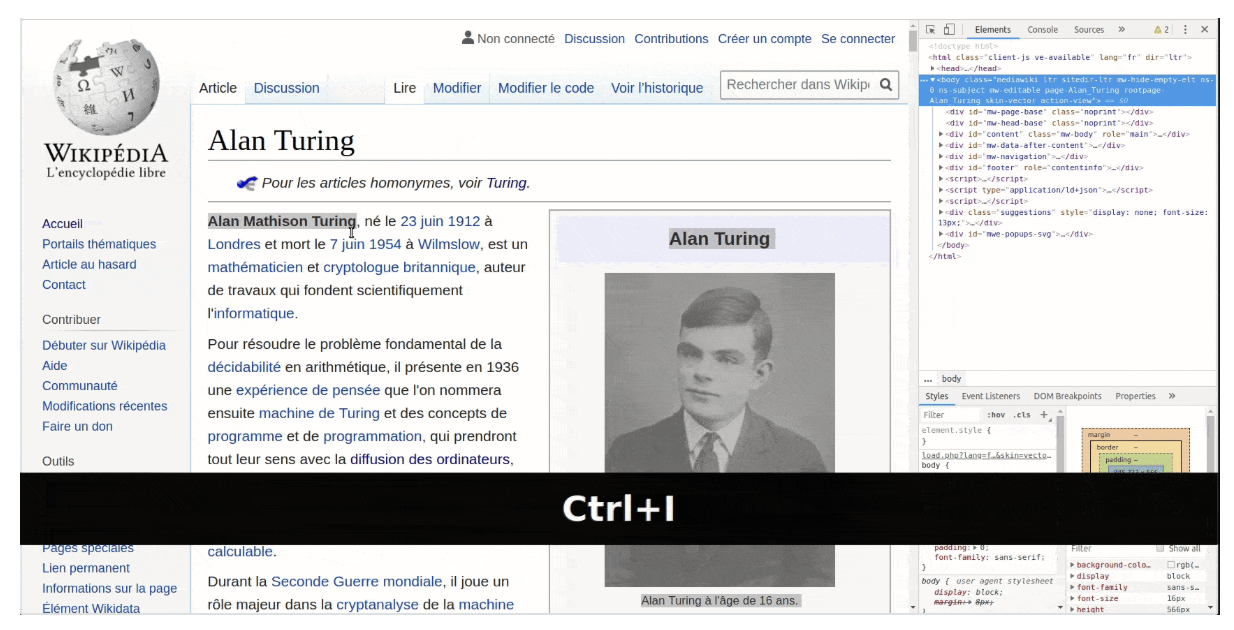
\includegraphics[width=10cm]{images/image09.png}
\end{center}

\subsection{Changer l'emplacement de l'inspecteur}
Ouvrez le panel en faisant Ctrl + Maj + p et entrez la position : right ou bottom et pressez entrée :
\begin{center}
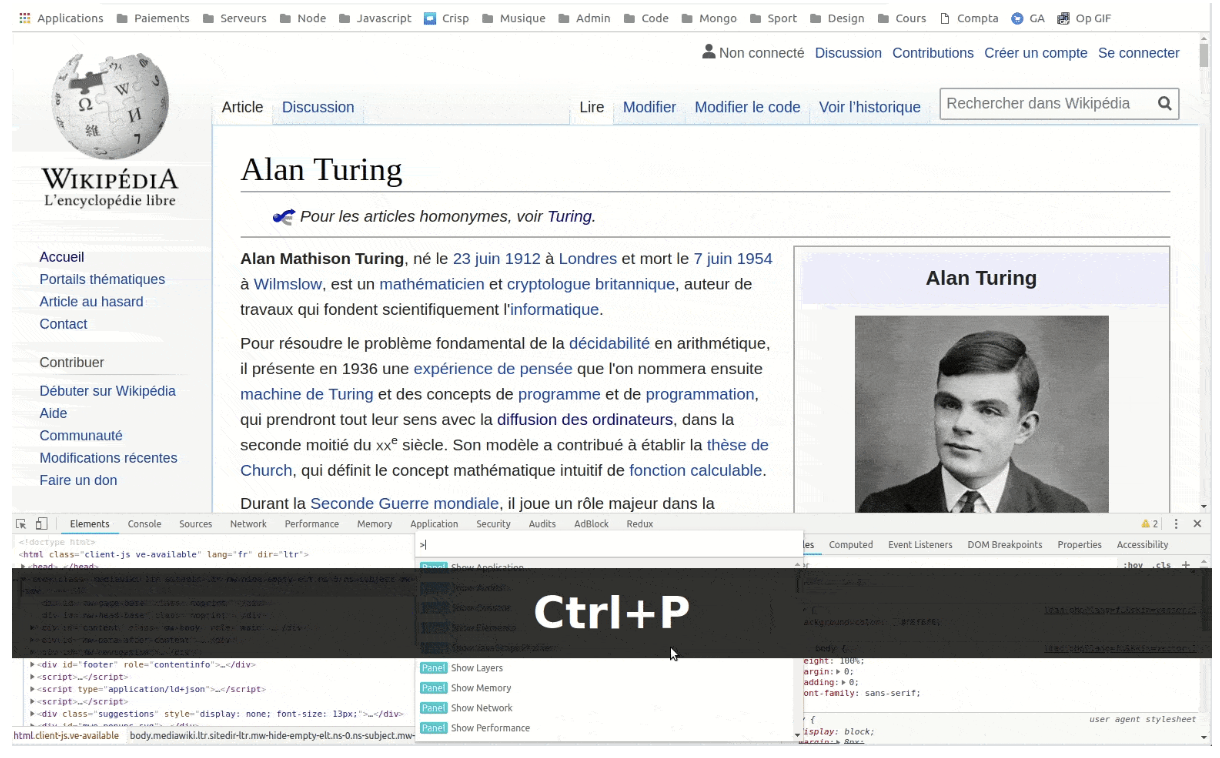
\includegraphics[width=10cm]{images/image10.png}
\end{center}

Vous pouvez ensuite voir les styles appliqués à un élément dans l'onglet Styles.

Vous pouvez également utiliser l'onglet Elements pour sélectionner d'autres éléments et voir les styles qui leur sont appliqués.

\subsection{De nouveaux raccourcis Emmet}
Nous avions vu * et > avec Emmet.

Pour rappel le premier permet de multiplier l'élément précédent par le chiffre passé après.

Le second permet d'imbriquer un élément dans le premier.

Nous allons voir + qui permet d'ajouter un élément au même niveau :

\begin{center}
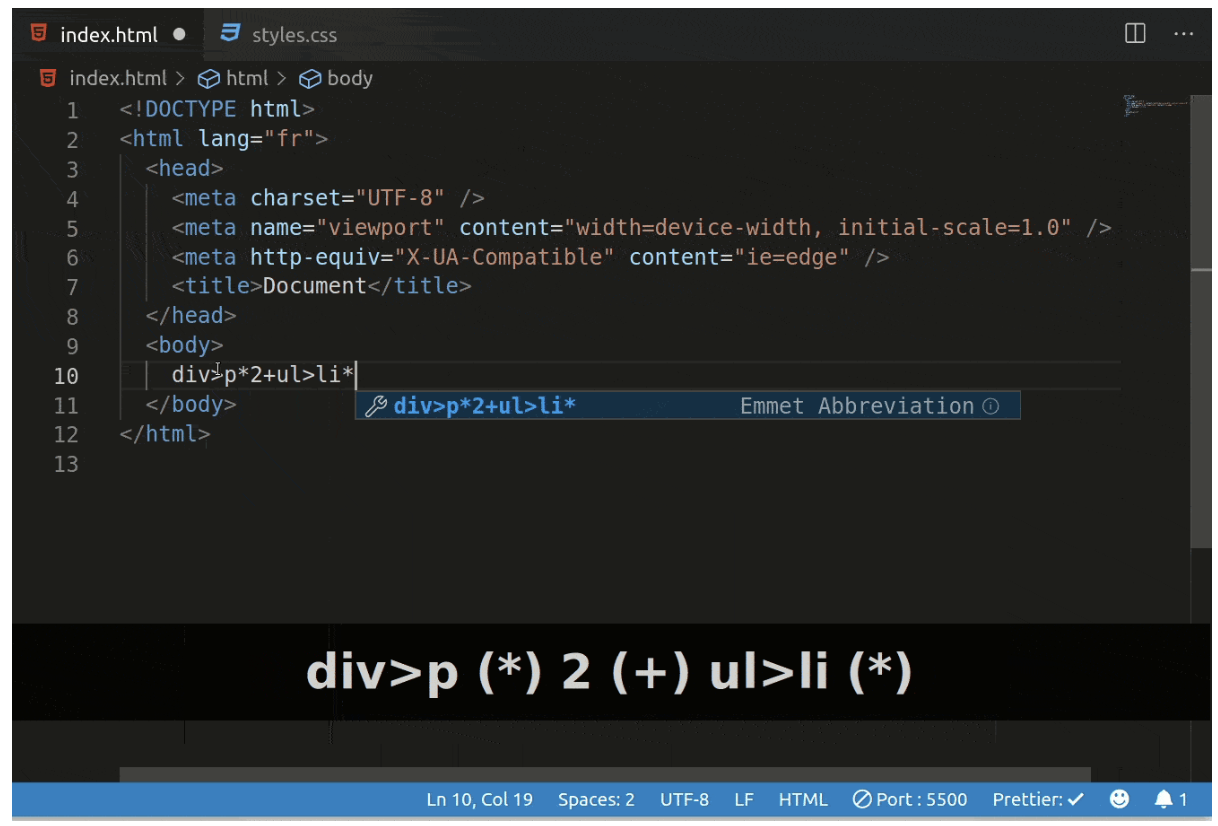
\includegraphics[width=10cm]{images/image11.png}
\end{center}

%%%%%%%%%%%%%%%%%%%%%%%%%%%%%%%%%%%%%%%%%%%%%%%%%%%%%%%%%%%%%%%%%%%%%%%%%%%%%%%%%

\section{Mise en forme du texte}
Dans cette leçon, nous allons voir comment modifier le style des textes en utilisant du CSS.

Police de caractères avec font-family
En typographie, une fonte de caractères est un ensemble de représentations visuelles de caractères, d'une même police d'écriture, de même style, corps et graisse.

Le corps est la taille d'une fonte de caractères, mesurée en points typographiques.

La graisse est l'épaisseur d'un trait ou d'un caractère.

Une police de caractère est l'ensemble des déclinaisons d'un même caractère.

Une déclinaison est donc une fonte. Par exemple, la police de caractères Times New Roman, est constituée d'une fonte romaine, d'une fonte italique, d'une fonte grasse et d'une fonte grasse italicisée.

font-family permet de définir une police ou une liste de polices.

Le navigateur n'appliquera une police de caractères que si elle est disponible, sinon, il utilisera une police par défaut.

Les polices Web dites sûres sont celles qui sont disponibles sur tous les systèmes et dans tous les navigateurs : Arial, Courrier New, Georgia, Times New Roman, Trebuchet MS et Verdana en sont des exemples.

Les polices se divisent en 5 familles génériques :

1 - serif : Polices avec fioritures.

2 - sans-serif : Les polices qui n'ont pas d'empattements

3 - monospace : Les polices dans lesquelles chaque caractère a la même largeur.

4 - cursive : Les polices qui ressemblent à de l'écriture manuscrite.

5 - fantasy : Les polices décoratives.

Vous pouvez déclarer une liste de polices :

font-family: "Times New Roman", Times, serif;
Copier
Dans ce cas la première sera appliquée, et si elle n'est pas disponible la deuxième, et si elle n'est pas disponible la famille de polices génériques serif.

Voici quelques exemples :


Vous pouvez trouver des polices gratuites sur https://www.fontsquirrel.com/ et https://www.dafont.com/fr/.

Taille de police avec font-size
La taille des polices de caractères est définie par la propriété font-size.

Elle accepte la plupart des unités de valeurs que nous étudierons dans la prochaine leçon. Mais voyons la plus utilisée, les pixels :

body {
  font-size: 20px;
}
Copier
Ici nous fixons à 20 le nombre de pixels souhaités pour la hauteur de tous les textes dans body.

La propriété font-size d'un élément est héritée de son parent. C'est-à-dire de l'élément dans lequel il est imbriqué.

Par défaut, tous les éléments ont une taille de police de 16px.

En effet, tous les éléments sont inclus dans l'élément <html>, et c'est la taille de la police qui est fixée par défaut pour cet élément dans tous les navigateurs.

Certains autres éléments ont des tailles par défaut en HTML, par exemple h1 a une taille par défaut de 2 em, qui comme nous le verrons, équivaut par défaut à 32px.

Graisse de la police avec font-weight
Comme nous l'avons vu, la graisse en typographie est l'épaisseur d'un caractère.

Elle se définit avec font-weight.

Vous pouvez utiliser bold comme raccourci ou alors utiliser une valeur numérique entre 100 et 900.

Style de la police avec font-style
Vous pouvez mettre la police en italique avec font-style :

<p style="font-style: italic"">Italique</p>
Copier
Décoration du texte avec text-decoration
Vous pouvez décorer le texte avec text-decoration.

underline permet de le souligner.

overline de tracer une ligne au-dessus.

line-through de le barrer.

A noter que text-decoration est un raccourci pour trois propriétés text-decoration-line, text-decoration-style et text-decoration-color.

Les valeurs possibles pour text-decoration-line sont celles que nous avons vues.

Les valeurs possibles pour text-decoration-style sont solid, double, dotted, dashed et wavy.

Transformer du texte avec text-transform
Vous pouvez transformer la police avec text-transform.

Les valeurs possibles sont : uppercase (tout en majuscule), lowercase (tout en minuscule) et capitalize (première lettre des mots en majuscule).

Hauteur de ligne
Il est possible de définir la hauteur de chaque ligne de texte avec line-height.

Vous pouvez passer une hauteur en pixels (ou toute autre unité de mesure que nous verrons) mais aussi juste un nombre qui sera alors un multiplicateur.

La hauteur de ligne recommandée est entre 1.5 et 2.

Espacement entre les lettres et les mots
Il est possible de définir l'espacement entre les lettres et les mots avec letter-spacing et word-spacing.

Vous pouvez définir la taille des espacements en px ou dans les autres unités de mesure que nous verrons dans la leçon suivante.

Exemples des mises en forme
Exceptionnellement les exemples utilisent du style en ligne mais uniquement pour que vous puissiez bien visualiser.

N'oubliez pas que ce n'est pas la méthode recommandée.


\end{document}

